\documentclass[12pt]{article}
\usepackage{hyperref}
\usepackage{graphicx}
\usepackage[toc,page]{appendix}
\graphicspath{ {pictures/} }
\usepackage[english]{babel}
\setlength{\parindent}{0em}
\setlength{\parskip}{1em}
\usepackage[margin=0.75in]{geometry}
\usepackage{fancyvrb}
\fvset{
	numbers=left
}


\title{MMEA User's Guide}
\author{Lukas Turcani}
\begin{document}

\begin{titlepage}
	\maketitle
\end{titlepage}

\tableofcontents
\newpage
\section{Introduction}
MMEA (MacroMolecular Evolutionary Algorithm) is a genetic algorithm (GA) for chemistry. It aims to be as general as possible, being suitable for use with any class of molecules. While it does not support all types of molecules out of the box, it is designed to be easily extended. This is made easier by being written in Python. For notes on how to extend MMEA to a new class of molecules or add GA operations, see the developer's guide.

\section{Installing MMEA}

\section{Input Files}
To run MMEA you need to use an input file. These contain all the details required to start a GA calculation. Among other things, this may include things like which fitness function you want to use, the number of generations MMEA should make and how big the population should be.

Using an example, the format and structure of input files is explained in section \ref{input_files_format_and_structure}. A guide to finding out what GA operations and tools are available is in section \ref{Finding available functions and their arguments.}. Examples of input files and accompanied explanations of what each line does are provided in section \ref{examples}.

\subsection{Format and structure.}
\label{input_files_format_and_structure}

The input file consists of a sequence of commands. Each command defines a variable or a function used by MMEA. If the command defines a function used by MMEA it must also define any parameters necessary to use the function. It does not have to define any default initialized parameters, though it may if desired. Commands can be written across multiple lines and terminate when the last parameter is defined. This means that 
\begin{Verbatim}
generational_select_func; 
stochastic_sampling; 
use_rank=True
\end{Verbatim}
and
\begin{Verbatim}
generational_select_func; stochastic_sampling; use_rank=True
\end{Verbatim}
define the same command. Notice there is no semicolon at the end of a command, it is only used to separate the parameters.

Any lines consisting of only whitespace or beginning with ``\#" are ignored.

There are two kinds of command in the input file. The first kind has the form
\begin{verbatim}
keyword; function_name; param1=val1; param2=val2; param3=val3
\end{verbatim}
For example, 
\begin{verbatim}
generational_select_func; stochastic_sampling; use_rank=True
\end{verbatim}
This means that the keyword is ``generational\_select\_func", the function name is ``stochastic\_sampling", parameter 1's name is ``use\_rank" and its value is ``True". As you can see, in this there is only 1 parameter name-value pair.

Commands with this format define functions used by MMEA. It is called the ``function definition format". The function will correspond to the various GA operations, such as crossover, mutation and selection or to things like the fitness function or optimization function (which optimizes the geometry of molecules created by MMEA). The words which make up the command are separated by a semicolon. Recall that the last word of a command is not followed by a semicolon. 

The keyword defines which GA operation the command describes. For example, in the command above the keyword ``generational\_select\_func" signifies that the command defines which function is to be used for selecting members of the next generation. The keyword in the command
\begin{verbatim}
parent_select_func; crossover_roulette
\end{verbatim} 
is ``parent\_select\_func", which signifies that the command defines the function used for selecting parents for crossover. A list of valid keywords is described in section \ref{list and explanation of valid keywords.}.

The parameter ``function\_name" is the name of the function which is to carry out the role designated by the keyword. This must correspond to the name of a function defined within MMEA. For example, if the keyword is ``generational\_select\_func" then ``stochastic\_sampling" or ``roulette" are both valid values for ``function\_name", because the module ``selection.py" within MMEA defines functions with these names. Indeed, any function defined within this module can be used as the selection function. Finding valid function names without looking at the source code is described in section \ref{Finding available functions and their arguments.}.

Finally, in the command above ``param1" and ``val1" correspond to ``use\_rank" and ``True", respectively. As mentioned before ``stochastic\_sampling" is the name of a function defined within the ``selection.py" module. As is usual for Python functions, it takes arguments. Looking at ``stochastic\_sampling()" within ``selection.py" it can be seen that its arguments are ``cls" and ``population" and its keyword arguments are ``elitism" (defaults to ``False"), ``truncation" (defaults to ``False"), ``duplicates" (defaults to ``False") and ``use\_rank" (defaults to ``False").

In the case of selection functions the first two arguments (``cls" and ``population") are dealt with automatically by MMEA. If the user wants to use one of the selection functions they have to provide values to any of the remaining arguments in the form ``param1=val1". The order in which they are given in the input file does not matter. If the user wants to change the default values of any of the function's keyword arguments, they may add them to the command using the same notation. Keyword arguments otherwise do not have to be provided in the input script and will be default initialized to whatever is defined within the source code of MMEA. All of this holds true for other functions defined in the input file, not just selection functions. How a user can easily view what functions and parameters are available, as well as what they mean, is addressed in section \ref{input_files_valid_parameters}.

When the user provides the value of a parameter, it must reflect its type. For example if a parameter wanted an a list of numbers then
\begin{verbatim}
param=[1,2,3,4]
\end{verbatim}
if it wanted a string
\begin{verbatim}
param="this is a string"
\end{verbatim}
or if it wanted a the name of a function or class defined within MMEA
\begin{verbatim}
param=some_mmea_function_name
\end{verbatim}
In essence it must be provided as valid Python syntax.

All keywords should be defined in the input file once. The exception to this is ``mutation\_func". It is quite possible that during a GA run the user's wishes to use multiple mutation operations. As a result it is perfectly reasonable to include multiple commands with the keyword  ``mutation\_func". When this is done, the user must also include the line 
\begin{verbatim}
mutation_weights=[0.1, 0.45,0.45]$
\end{verbatim}
This line tells MMEA that when a mutation is to be performed it should select the first mutation function defined in the input file with a 0.1 probability and the second and third mutation functions defined in the input file with a 0.45 probability. The probabilities can of course be modified by the user. The only requirements are that the probabilities sum to 1 and that the number of elements in the array and the number of mutation functions defined in the input file is the same.

There is a second kind of non-comment line in the input file of MMEA. These lines have the form
\begin{verbatim}
keyword=val$
\end{verbatim}
As you can see, these are much simpler. They define basic constants relevant to the GA. As a result, this is called the ``constant definition format". This includes things like population size, number of crossovers carried out during each generation and so on. It is merely the keyword, a ``=" and the value. No spaces. Valid keywords for these lines are discussed in section \ref{input_files_valid_parameters}.

\subsection{Valid input values.}
\label{input_files_valid_parameters}
In order to prevent the need to continuously update this documentation when a new function is added to MMEA, only valid keywords are described here. However, this does not mean a user has to go into the source code to find out what functions they have at their disposal. This section also describes how MMEA can be made to output valid function names and parameters for each keyword.
\subsubsection{List and explanation of valid keywords.}
\label{list and explanation of valid keywords.}
Here is a list of valid keywords, the type of line formatting the keyword requires and which arguments do not need to be provided to the functions. Recall in section \ref{input_files_format_and_structure} the selection function did not require the ``population" argument to be provided explictily in the input file. Other functions, such as crossover functions do not require other parameters to be provided. The format here is:
\\
\\
\textbf{keyword} - \textit{line format} - \textbf{excluded\_param1, excluded\_param2} - Explantion of keyword.
\\
\\
The keywords are:
\\
\\
\textbf{init\_func} - \textit{function definition format} - \textbf{ga\_tools} - The function used to create the initial population.
\\
\\
\textbf{generational\_select\_func} - \textit{function definition format} - \textbf{population} - The function used to select members of the next generation.
\\
\\
\textbf{parent\_select\_func} - \textit{function definition format} - \textbf{population} - The function used to select parents for crossover.
\\
\\
\textbf{mutant\_select\_func} - \textit{function definition format} - \textbf{population} - The function used to select individuals for mutation.
\\
\\
\textbf{crossover\_func} - \textit{function definition format} - \textbf{marco\_mol1, macro\_mol2} - The function which carries out the crossover operation.
\\
\\
\textbf{mutation\_func} - \textit{function definition format} - \textbf{macro\_mol} - The function which carries out the mutation operation.
\\
\\
\textbf{opt\_func} - \textit{function definition format} - \textbf{macro\_mol} - The function which optimizes the geometry of the molecules.
\\
\\
\textbf{fitness\_func} - \textit{function definition format} - \textbf{macro\_mol, population} - The function which calculates fitness.
\\
\\
\textbf{num\_generations} - \textit{constant definition format} - The number of generations which MMEA will create.
\\
\\
\textbf{num\_mutations} - \textit{constant definition format} - The number of mutations MMEA will carry out each generation.
\\
\\
\textbf{num\_crosses} - \textit{constant definition format} - The number of crossover operations MMEA will carry out each generation.
\\
\\
\textbf{pop\_size} - \textit{constant definition format} - The size of the population.
\\
\\
\textbf{mutation\_weights} - \textit{constant definition format} - The probability with which each mutation function defined in the input file will be used when a mutation operation is performed. Note that the form of this constant is an array. For example
\begin{verbatim}
mutation_weights=[0.1, 0.45,0.45]$
\end{verbatim}

\subsubsection{Finding available functions and their arguments.}
\label{Finding available functions and their arguments.}
In order to find out what functions MMEA offers for a given keyword, using a console go into the directory containing MMEA. 

Run the command 
\begin{verbatim}
python -m MMEA -h keyword
\end{verbatim}
where keyword is one of the valid function definition keywords defined in section \ref{list and explanation of valid keywords.}.


\includegraphics[scale=1]{console1}

MMEA will then output a list of valid functions, their description, and a list of their parameters.

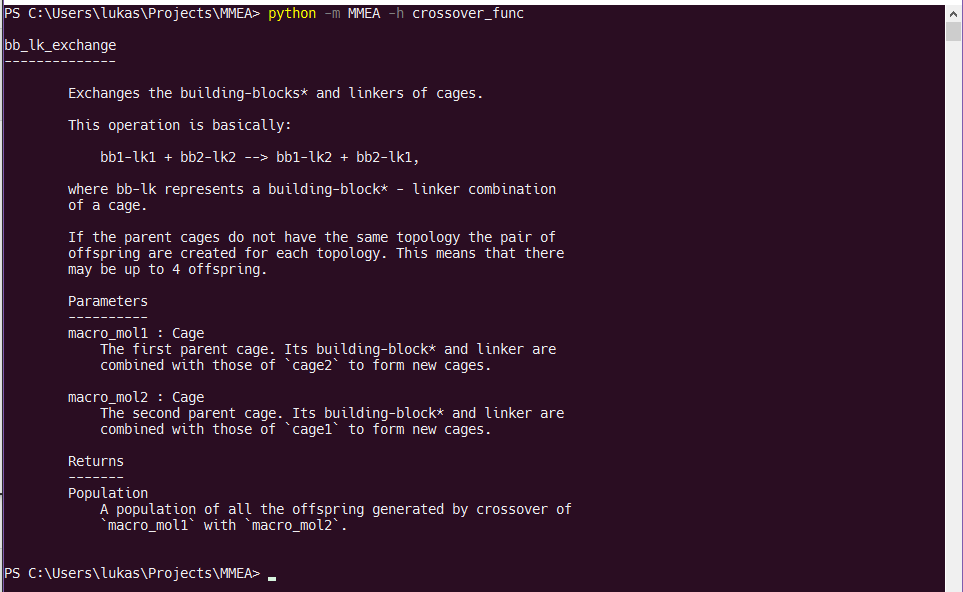
\includegraphics[scale=0.7]{console2}

In this example, the keyword ``crossover\_func" was used and the only available function was ``bb\_lk\_exchange" Other keywords will have more options available (and more may be added to this one). As you can see the only parameters the function takes are macro\_mol1 and macro\_mol2. As these are handled automatically by MMEA (\ref{list and explanation of valid keywords.}) no parameters should be provided in the input file. A valid line would look like
\begin{verbatim}
crossover_func; bb_lk_exchange$
\end{verbatim}

\subsection{Examples}
\label{examples}
Here are example input files followed by a line by line explanation of what they're doing.

\subsection{Example 1}
\label{example 1}
\begin{Verbatim}
##################################################################################
# Population initialization function.
##################################################################################

init_func; init_random_cages;
bb_db="/home/username/aldehydes_3f";
lk_db="/home/username/amines_2f";
topologies=[FourPlusSix, EightPlusTwelve]$

##################################################################################
# Selection function for selecting the next generation.
##################################################################################

generational_select_func; stochastic_sampling; use_rank=True$

##################################################################################
# Selection function for selecting parents.
##################################################################################

parent_select_func; crossover_roulette$

##################################################################################
# Selection function for selecting molecules for mutation.
##################################################################################

mutant_select_func; stochastic_sampling; duplicates=True$

##################################################################################
# Crossover function.
##################################################################################

crossover_func; bb_lk_exchange$

##################################################################################
# Mutation function 1.
##################################################################################

mutation_func; similar_bb;
database="/home/username/aldehydes_3f"$

##################################################################################
# Mutation function 2.
##################################################################################

mutation_func; similar_lk;
database="/home/username/amines_2f"$

##################################################################################
# When carrying mutations, chance that a given mutation function will be used.
##################################################################################

mutation_weights=[1/2,1/2]$

##################################################################################
# Optimization function.
##################################################################################

opt_func; macromodel_cage_opt;
macromodel_path="/home/username/program_files/schrodinger2016-3"$

##################################################################################
# Fitness function.
##################################################################################

fitness_func; cage; target_cavity=8; coeffs=[1,1,5,0,0];
energy_params={"key":("macromodel", 16, "/home/username/schrodinger2016-3")}$

##################################################################################
# Number of generations to create.
##################################################################################

num_generations=10$

##################################################################################
# Number of mutation operations to perform each generation.
##################################################################################

num_mutations=10$

##################################################################################
# Number of crossover operations to perform each generation.
##################################################################################

num_crossovers=15$

##################################################################################
# Size of the population.
##################################################################################

pop_size=20$
\end{Verbatim}

The first command runs from line 5 to 8. It has the keyword ``init\_func", which means that it defines the initialization function for the GA population. The initialization function is called ``init\_random\_cages". This function creates a population consisting of randomly assembled ``cage" molecules. The function takes the parameter ``bb\_db" which receives a string. The string is the path of a directory which holds monomers used for constructing the cages. The parameter ``lk\_db" has the same role. The parameter ``topologies" requires an array or list. The list contains the names of cage topologies defined within MMEA.

The second command is on line 14. The keyword ``generational\_select\_func" indicates that the command defines the selection function used for selecting the next generation.

\section{Running MMEA}

\subsection{From the command line.}


\section{Output}

\section{MMEA as a Library}

\end{document}